\documentclass[a4paper,12pt]{article}
\usepackage{amsmath,amsfonts,amssymb} % Math packages
\usepackage{mathtools} % For defining floor and ceiling functions
\usepackage{amsthm}    % Theorems
\usepackage{bm} 	   % Bold math
\usepackage{bbm}	   % More bold math?
\usepackage{array}     % Better tables
\usepackage{chemfig}   % chemical figures
\usepackage{physics}   % derivatives and partials
\usepackage{float}     % Better positioning [H]
\usepackage{framed}    % Framed boxes
\usepackage{geometry}  % Required for adjusting page dimensions and margins
\usepackage{graphicx}  % Include images
\usepackage{multirow}  % multicolumn tables
\usepackage{pgfplots}  % Create plots in latex
\usepackage{siunitx}   % SI unit system
\usepackage{listings}  % Code environments
\usepackage[shortlabels]{enumitem} %lets us change the enumeration to (a), (b), ...
\usepackage{booktabs}  % Better looking horizontal rules
\usepackage{makecell}  % Pre-formatting of column heads
\usepackage{hyperref}  % Clickable links
\renewcommand{\arraystretch}{1.6}

% Theorems and definitions
\theoremstyle{definition}
\newtheorem*{definition}{Definition}
\newtheorem*{proposition}{Proposition}
\newtheorem*{theorem}{Theorem}
\pgfplotsset{width=10cm,compat=1.9}

% Graph drawings
\usetikzlibrary{shapes,arrows,positioning,} % Graph arrows
\usetikzlibrary{automata,positioning,fit,shapes.geometric,backgrounds} % Node grouping

% stats commands
\newcommand{\E}{\mathbb{E}}
\newcommand{\Var}{\mathbb{V}\mathrm{ar}}
\newcommand{\Cov}{\mathbb{C}\mathrm{ov}}
\newcommand{\Risk}{\mathcal{R}}

% common number sets
\newcommand{\N}{\mathbb{N}}
\newcommand{\R}{\mathbb{R}}
\newcommand{\Q}{\mathbb{Q}}
\newcommand{\Z}{\mathbb{Z}}
\newcommand{\C}{\mathbb{C}}

% Cs stuff
\newcommand{\bigO}{\mathcal{O}}

% Indicator function
\newcommand{\Ind}[1]{\mathbbm{1}_{\{#1\}}}

\DeclarePairedDelimiter\ceil{\lceil}{\rceil}
\DeclarePairedDelimiter\floor{\lfloor}{\rfloor}
\DeclarePairedDelimiter\angleb{\langle}{\rangle}

\geometry{
	paper=a4paper, % Paper size, change to letterpaper for US letter size
	top=2.5cm, % Top margin
	bottom=2.5cm, % Bottom margin
	left=2.5cm, % Left margin
	right=2.5cm, % Right margin
	headheight=14pt, % Header height
	footskip=1.5cm, % Space from the bottom margin to the baseline of the footer
	headsep=1.2cm, % Space from the top margin to the baseline of the header
}

\lstset{
	basicstyle=\ttfamily,
	mathescape,
	inputencoding=utf8,
	escapeinside={\%*}{*)},
	literate={á}{{\'a}}1 {ã}{{\~a}}1 {é}{{\'e}}1 {É}{{\'E}}1 {è}{{\`e}}1 {à}{{\`a}}1,
	numbers=left,
	breaklines=true
}

\let\tss\textsuperscript % superscript macro
\let\oldtextbf\textbf
\renewcommand{\textbf}[1]{\oldtextbf{\boldmath #1}}

\newtheorem{exercise}{Exercise}[section]

\begin{document}
\title{Deep Learning}
\author{David Zhao}
\date{Febrary 9, 2023}
\maketitle

\section{Preface}
This paper is a learning documentation adapted/copied from the book \href{https://d2l.ai/}{Dive into Deep learning}.
Coding implementations are omitted (for now).

\section{Preliminaries}
\subsection*{AutoDifferentiation}

\subsection*{Linear Algebra}
\subsubsection*{Norms}
Some of the most useful operators in linear algebra are norms. Informally, the norm of a vector tells us how big it is.
Here, we are employing a notion of size that concerns the magnitude of a vector’s components (not its dimensionality).

A norm is a function $||\cdot||$ that maps a vector to a scalar and satisfies the following three properties:
\begin{enumerate}
    \item Given any vector $\mathbf{x}$, if we scale the vector by a scalar $\alpha \in \R$, its norm scales accordingly:

          \begin{align*}
              ||\alpha\mathbf{x}|| = |\alpha|||\mathbf{x}||
          \end{align*}

    \item For any vectors $\mathbf{x}$ and $\mathbf{y}$, norms must satisfy the triangle inequality:

          \begin{align*}
              ||\mathbf{x} + \mathbf{y}|| = ||\mathbf{x}|| + ||\mathbf{y}||
          \end{align*}

    \item The norm of a vector is nonnegative and vanishes if and only if the vector is zero:

          \begin{align*}
              ||\mathbf{x}|| > 0 \iff \mathbf{x} \neq 0
          \end{align*}

\end{enumerate}
For instance, the $l2$ norm measures the (Euclidean) length of a vector which we've all seen already in school when calculating the hypotenuse of a right triangle..
Formally, we know it as

\begin{align*}
    ||\mathbf{x}||_2 = \sqrt{\sum_{i=1}^{n}\mathbf{x}_i^2}
\end{align*}

The $l1$ norm is also popular and the associated metric is called the Manhattan distance. By definition, the
norm sums the absolute values of a vector's elements:

\begin{align*}
    ||\mathbf{x}||_1 = \sum_{i=1}^{n}|\mathbf{x}_i|
\end{align*}

Both the $l_1$ and $l_2$ norms are special cases of the more general norms:
\begin{align*}
    ||\mathbf{x}||_p = \left({\sum_{i=1}^{n}\mathbf{x}_i^p}\right)^{1/p}
\end{align*}
\subsection*{Chain Rule}
Let $y = f(\mathbf{u})$ such that $\forall i, \mathbf{u}_i = g_i(\mathbf{x})$ where $\mathbf{u} = (u_1, u_2, \ldots, u_m)$ and $\mathbf{x} = (x_1, x_2, \ldots, x_n)$. \\
Then
\begin{align*}
    \frac{\partial y}{\partial x_i} = \frac{\partial y}{\partial u_1}\frac{\partial u_1}{\partial x_i} + \ldots + \frac{\partial y}{\partial u_m}\frac{\partial u_m}{\partial x_i}
\end{align*}

\subsection*{Baye's Theorem}
Given any event A and B such that $P(B) \neq 0$,
\begin{align*}
    P(A|B) = \frac{P(B|A)P(A)}{P(B)}
\end{align*}

\subsection*{Expectations}

\section{Linear Neural Networks for Regression}
We assume that the relationship between features $\mathbf{x}$ and target $y$ is approximately linear, i.e,

\begin{align*}
    E[Y|X=\mathbf{x}] = x_1w_1 + \ldots + x_dw_d + b
\end{align*}
where $d$ is the \textit{feature dimensionality}, and $b$ is the \textit{bias}. As such,

\begin{align*}
    \hat{y} & = \mathbf{w}^T\mathbf{x} + b
            & = \mathbf{Xw} + b
\end{align*}

In essence, our goal is to find parameters $\mathbf{w}$ and $b$ such that our prediction error is
minimized for new data examples that are sampled from the same distribution X.
\begin{figure}[h]
    \centering
    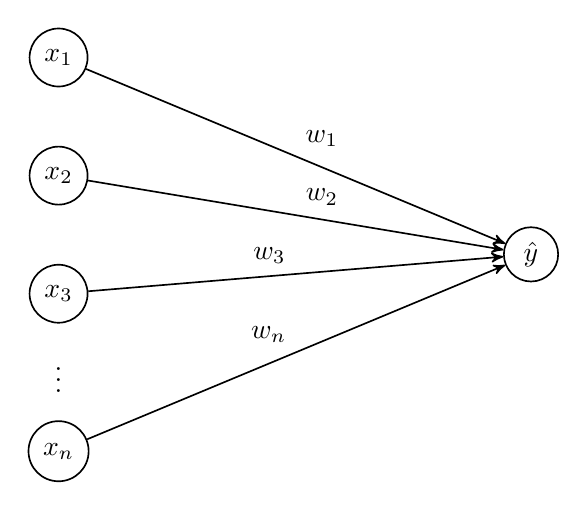
\begin{tikzpicture}[->, >=stealth', auto, semithick, node distance=3cm]
        \tikzstyle{every state}=[fill=white,draw=black,thick,text=black,scale=1]
        \node[draw, circle]    (x1) at (0,0)        {$x_1$};
        \node[draw, circle]    (x2) at (0,-1.5)     {$x_2$};
        \node[draw, circle]    (x3) at (0,-3)       {$x_3$};
        \node[draw, circle]    (xn) at (0,-5)       {$x_n$};
        \node[draw, circle]    (y) at (6,-2.5)      {$\hat{y}$};
        \begin{scope}[on background layer]
        \end{scope}
        \path
        (x1) edge[]	node{$w_1$}	(y)
        (x2) edge[]	node{$w_2$}	(y)
        (x3) edge[]	node{$w_3$}	(y)
        (x3) -- node[auto=false]{\vdots} (xn)
        (xn) edge[]	node{$w_n$}	(y);
    \end{tikzpicture}
    \caption{Linear Regression Model with feature dimensionality $n$}
\end{figure}
\subsection*{Loss Function}
Naturally, our model requires an objective measure of how well or unwell it fits the training data.
Loss functions fill in this role by quantifying the distance between the \textit{observed} and \textit{predicted}
labels. The most commonly used loss function is the squared error.

\begin{align*}
    l^{(i)}(\mathbf{w},b) = \frac{1}{2}(\hat{y}^{(i)}-\mathbf{y}^{(i)})^2
\end{align*}
Note that the presence of the constant coefficient $\frac{1}{2}$ is notationally convenient as it disappears when we
take the derivative of the loss function. Also notice that large differences between estimates $\hat{y}^{(i)}$
and targets $\mathbf{y}^{(i)}$ lead to larger contributions due to the function's quadratic form. In fact, while
it does encourage our model to avoid sizeable errors, it also yields an excessive sensitivity to anomalous data.
To evaluate our model's performance over entire the dataset of $n$ examples, we simply take the average of
the losses on the training set:
\begin{align*}
    L^{(i)}(\mathbf{w},b) = \frac{1}{n}\sum_{i=1}^{n}\frac{1}{2}(\hat{y}^{(i)}-\mathbf{y}^{(i)})^2
\end{align*}
Our goal is to find parameters $\mathbf{w}^*$ and $b^*$ that can minizmize the total loss across all examples.

\subsection*{Minibatch Stochastic Gradient Descent}

\begin{align*}
    (\mathbf{w},b) & \leftarrow (\mathbf{w},b) - \frac{\eta}{|\beta|}\sum_{i\in\beta_i}\frac{\partial}{\partial(\mathbf{w},b)}l^{(i)}(\mathbf{w},b)                                                                                                                   \\
    \mathbf{w}     & \leftarrow \mathbf{w} - \frac{\eta}{|\beta|}\sum_{i\in\beta_i}\frac{\partial}{\partial\mathbf{w}}l^{(i)}(\mathbf{w},b) = \mathbf{w}- \frac{\eta}{|\beta|}\sum_{i\in\beta_i}\mathbf{x}^{(i)}(\mathbf{w}^T\mathbf{x}^{(i)} + b - \mathbf{y}^{(i)}) \\
    b              & \leftarrow b - \frac{\eta}{|\beta|}\sum_{i\in\beta_i}\frac{\partial}{\partial b}l^{(i)}(\mathbf{w},b) = \mathbf{w}- \frac{\eta}{|\beta|}\sum_{i\in\beta_i}(\mathbf{w}^T\mathbf{x}^{(i)} + b - \mathbf{y}^{(i)})
\end{align*}


\subsection*{Normal Distribution and Squared Loss}
So far we have given a fairly functional motivation of the squared loss objective: the optimal parameters return the conditional expectation
whenever the underlying pattern is truly linear, and the loss assigns outsize penalties for outliers. We can also provide a more formal motivation for the squared loss objective by making probabilistic assumptions about the distribution of noise.

To begin, recall that a normal distribution with mean $\mu$ and variance $\sigma^2$ (standard deviation $\sigma$) is given as

\begin{align*}
    p(x) = \frac{1}{\sqrt{2\pi\sigma^2}}\exp({-\frac{1}{2\sigma^2}(x-\mu)^2})
\end{align*}

One way to motivate linear regression with squared loss is to assume that observations arise from noisy measurements, where the noise is normally distributed as follows:

\begin{align*}
    y = \mathbf{w}^T\mathbf{x} + b + \epsilon &  & \textrm{where}\ \epsilon \sim \mathcal{N}(0,\,\sigma^{2})
\end{align*}

Thus, we can now write out the likelihood of seeing a particular $y$ for a given $\mathbf{x}$ via

\begin{align*}
    P(y|\mathbf{x}) = \frac{1}{\sqrt{2\pi\sigma^2}}\exp({-\frac{1}{2\sigma^2}(y - \mathbf{w}^T\mathbf{x} - b)^2})
\end{align*}

As such, the likelihood factorizes. According to the \textit{principle of maximum likelihood}, the best values of parameters $\mathbf{w}$ and $b$
are those that maximize the likelihood of the entire dataset:

\begin{align*}
    P(y|X) = \prod_{i=1}^{n}P(\mathbf{y}^{(i)}|\mathbf{x}^{(i)})
\end{align*}

since all pairs $(\mathbf{x}^{(i)},y^{(i)})$ were drawn independently of each other. But, maximizing the product of exponential
functions is awkward. Instead, we minimize the negative log-likelihood:

\begin{align*}
    -\log(y|X) & = -log(\prod_{i=1}^{n}P(\mathbf{y}^{(i)}|\mathbf{x}^{(i)}))                                                               \\
               & = \sum_{i=1}^{n} \frac{1}{2}\log(2\pi\sigma^2) + \frac{1}{2\sigma^2}(\mathbf{y}^{(i)}-\mathbf{w}^T\mathbf{x}^{(i)} - b)^2
\end{align*}

It follows that minimizing the square error loss is equivalent to the maximum likelihood estimation of a linear model
under additive Gaussian noise.

\subsection*{Generalization}
The phenomenon of our model fitting closer to the training model than to the underlying distribution is called \textit{overfitting}.
Instead, our goal is to train our model in such a way that it may find a generalizable pattern and make correct
predictions about previously unseen data.
\subsubsection*{Training Error \& Generalization Error}
In standard supervised learning setting, we assume the training and testing data to be drawn independently from
identical distributions (i.e. \textit{IID} assumption).
Training error ($R_{emp}$) is a statistic calculated on the training dataset:

\begin{align*}
    R_{emp}[X,\mathbf{y},f] = \frac{1}{n}\sum_{i=1}^{n}l(\mathbf{x}^{(i)},\mathbf{y}^{(i)},f(\mathbf{x})^{(i)})
\end{align*}

Generalization error ($R$) is an expectation taken with respect to the underlying distribution:

\begin{align*}
    R[p,f] = E_{(\mathbf{x},y)\sim P[l(\mathbf{x},y,f(\mathbf{x})]} = \int\int l(\mathbf{x},y,f(\mathbf{x}))p(\mathbf{x},y)d\mathbf{x}dy
\end{align*}

We are essentially taking the average value of the loss function over all possible pairs of inputs $\mathbf{x}$ and labels $y$ sampled from
the underlying distribution $P$, which amounts to integrating the loss function $l(\mathbf{x}, y f(\mathbf{x}))$ multiplied by the joint probability
density function $p(\mathbf{x}, y)$ over the input space $\mathbf{x}$ and the label space $y$.

Note that we can never measure $R$ exactly since the density function $p(\mathbf{x},y)$ has a form that can almost never
be precisely known. Moreover, since we cannot sample an infinite stream of data points, we must resort to estimating
the generalization error by applying our model to an independent test set that is withheld from our training set.
\subsubsection*{Model Complexity}
Intuitively, when we have simple models mixed with abundant data, the training and generalization error tend to be close.
Conversely, we can expect more a complex model and/or fewer examples to cause our training error to diminish, but the
generalization error to grow. Error on the holdout data, i.e. the validation set, is called the \textit{validation error}.

\subsubsection*{Polynomial Curve Fitting}
\subsubsection*{Cross Validation}
In cases when we are dealt with scarce training data, it is likely that we often lack enough hold out data to form a validation
set. A popular solution is to use \textit{K-fold cross-validation} where the training data is first partitioned into $k$ disjoints
sets. Then, we perform a total of $k$ training/validation steps, each time training on $k-1$ sets and validating on the remaining unused set.
Finally, we average the training and validation errors over the results obtained from our $k$ experiments.
\subsection*{Weight Decay}
Recall that we can always mitigate overfitting by collecting more training data. However, gathering more data is often costly, time consuming,
etc. Therefore, we introduce our first \textit{regularization} technique known as \textit{weight decay}.

Note that we may also limit model complexity by tweaking the degree of our fitted polynomial. However, even small
changes in degree can dramatically increase model complexity, hence motivating our necessity for a more fine-tuning method, i.e. weight decay.

\subsubsection*{Norms \& Weight Decay}

\begin{align*}
    \mathbf{w} & \leftarrow (1-\eta\lambda)\mathbf{w} - \frac{\eta}{|\beta|}\sum_{i\in\beta_i}\frac{\partial}{\partial\mathbf{w}}l^{(i)}(\mathbf{w},b) = \mathbf{w}- \frac{\eta}{|\beta|}\sum_{i\in\beta_i}\mathbf{x}^{(i)}(\mathbf{w}^T\mathbf{x}^{(i)} + b - \mathbf{y}^{(i)}) \\
\end{align*}


\section{Linear Neural Networks for Classification}

\subsection*{Classification}
To get our feet wet, let's start with a simple image classification problem. Here, each input consists of a $2\times2$
grayscale image. We can represent each pixel value with a single scalar, giving us four features $x_1, x_2, x_3, x_4$.
Further, let's assume that each image belongs to one among the categories “cat”, “chicken”, and “dog”.
\newline
In general, classification problems do not come with natural orderings among the classes. Fortunately, statisticians long ago invented a
simple way to represent categorical data: the \emph{one-hot encoding}. A one-hot encoding is a vector with as many components as we have
categories. The component corresponding to a particular instance’s category is set to 1 and all other components are set to 0. In our case,
a label would be a three-dimensional vector, with $(1,0,0)$ corresponding to “cat”, $(0,1,0)$ to “chicken”, and $(0,0,1)$ to “dog”.
\subsection*{Linear Model}

\begin{align*}
    o_1 & = x_1 w_{11} + x_2 w_{12} + x_3 w_{13} + x_4 w_{14} + b_1, \\
    o_2 & = x_1 w_{21} + x_2 w_{22} + x_3 w_{23} + x_4 w_{24} + b_2, \\
    o_3 & = x_1 w_{31} + x_2 w_{32} + x_3 w_{33} + x_4 w_{34} + b_3.
\end{align*}



Assuming a suitable loss function, we could try, directly, to minimize the difference between
and the labels
. While it turns out that treating classification as a vector-valued regression problem works surprisingly well, it is nonetheless lacking in the following ways:
\begin{itemize}
    \item There is no guarantee that the outputs $\sigma_i$ sum up to 1 in the way we expect probabilities to behave.
    \item There is no guarantee that the outputs $\sigma_i$ are even nonnegative, even if their outputs sum up to 1, or that they do not exceed 1
\end{itemize}
\subsection*{Softmax}

\begin{align*}
    \hat{\mathbf{y}} = \mathrm{softmax}(\mathbf{o}) \quad \text{where} \quad \hat{y}_i = \frac{\exp(o_i)}{\sum_j \exp(o_j)}.
\end{align*}


\subsection*{Log-Likelihood}

\begin{align*}
    P(\mathbf{Y} \mid \mathbf{X}) = \prod_{i=1}^n P(\mathbf{y}^{(i)} \mid \mathbf{x}^{(i)}).
\end{align*}


\begin{align*}
    l(\mathbf{y},\mathbf{\hat{y}}) = -\sum_{j=1}^{q}y_j \log \hat{y_j}
\end{align*}


\subsection*{Softmax and Cross-Entropy Loss}

\begin{align*}
    l(\mathbf{y}, \hat{\mathbf{y}}) & =  - \sum_{j=1}^q y_j \log \frac{\exp(o_j)}{\sum_{k=1}^q \exp(o_k)}   \\
                                    & = \sum_{j=1}^q y_j \log \sum_{k=1}^q \exp(o_k) - \sum_{j=1}^q y_j o_j \\
                                    & = \log \sum_{k=1}^q \exp(o_k) - \sum_{j=1}^q y_j o_j.
\end{align*}



\begin{align*}
    \partial_{o_j} l(\mathbf{y}, \hat{\mathbf{y}}) = \frac{\exp(o_j)}{\sum_{k=1}^q \exp(o_k)} - y_j = \mathrm{softmax}(\mathbf{o})_j - y_j.
\end{align*}

\section{Multilayer Perceptrons}
Recall in section 3, we described affine transformations as linear transformations with added bias. This model maps inputs directly to
outputs via a single affine transformation, followed by a softmax operation. However, linearity is often a strong assumption.
\subsection*{Limitations of Linear Models}
Linearity implies the weaker law of \textit{monotonicity} i.e. any increase in inputs must always correspond to an increase in our model's
output (positive weights), or a decrease in our model's output (negative weights). Often times, linearity becomes too strong of an assumption
to be applied to problems that require more specific modelling. Suppose for example we want to predict whether an individual will repay loan
based on their salary. Although this relationship is monotonic, it is perhaps not linear as an increase in income from \$0 to \$50,000 likely
corresponds to a higher likelihood of repayment than an increase from \$1 million to \$1.05 million. As such, it may be preferable to
post-process our outcome by using a logarithmic map, to make linearity a more plausible assumption.
\subsection*{Incorporating Hidden Layers}
We overcome the limitations of linearity by incorporating one or more hidden layers. The most common way to do this is to stack many fully
connected layers on top of each other. We can think of the first $L-1$ layers as our representation and the final layer as our linear predictor.
This architecture is commonly called a \textit{multilayer preceptron} or \textit{MLP}.

\subsection*{From Linear to Nonlinear}
\begin{figure}[h]
    \centering
    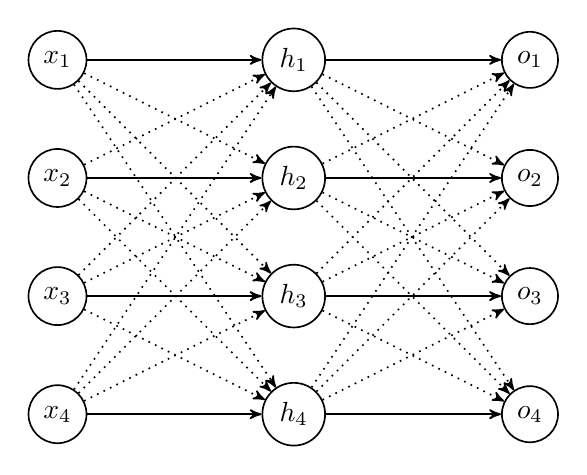
\begin{tikzpicture}[->, >=stealth', auto, semithick, node distance=3cm]
        \tikzstyle{every state}=[fill=white,draw=black,thick,text=black,scale=1]
        \node[draw, circle]    (x1) at (0,0)        {$x_1$};
        \node[draw, circle]    (x2) at (0,-1.5)     {$x_2$};
        \node[draw, circle]    (x3) at (0,-3)       {$x_3$};
        \node[draw, circle]    (x4) at (0,-4.5)     {$x_4$};
        \node[draw, circle]    (h1) at (3,0)        {$h_1$};
        \node[draw, circle]    (h2) at (3,-1.5)     {$h_2$};
        \node[draw, circle]    (h3) at (3,-3)       {$h_3$};
        \node[draw, circle]    (h4) at (3,-4.5)     {$h_4$};
        \node[draw, circle]    (o1) at (6,0)        {$o_1$};
        \node[draw, circle]    (o2) at (6,-1.5)     {$o_2$};
        \node[draw, circle]    (o3) at (6,-3)       {$o_3$};
        \node[draw, circle]    (o4) at (6,-4.5)     {$o_4$};
        \begin{scope}[on background layer]
        \end{scope}
        \path
        (x1) edge[]	node{}	        (h1)
        (x1) edge[dotted]	node{}	(h2)
        (x1) edge[dotted]	node{}	(h3)
        (x1) edge[dotted]	node{}	(h4)
        (x2) edge[dotted]	node{}	(h1)
        (x2) edge[]	node{}	        (h2)
        (x2) edge[dotted]	node{}	(h3)
        (x2) edge[dotted]	node{}	(h4)
        (x3) edge[dotted]	node{}	(h1)
        (x3) edge[dotted]	node{}	(h2)
        (x3) edge[]	node{}	        (h3)
        (x3) edge[dotted]	node{}	(h4)
        (x4) edge[dotted]	node{}	(h1)
        (x4) edge[dotted]	node{}	(h2)
        (x4) edge[dotted]	node{}	(h3)
        (x4) edge[]	node{}	        (h4)
        (h1) edge[]	node{}	        (o1)
        (h1) edge[dotted]	node{}	(o2)
        (h1) edge[dotted]	node{}	(o3)
        (h1) edge[dotted]	node{}	(o4)
        (h2) edge[dotted]	node{}	(o1)
        (h2) edge[]	node{}	        (o2)
        (h2) edge[dotted]	node{}	(o3)
        (h2) edge[dotted]	node{}	(o4)
        (h3) edge[dotted]	node{}	(o1)
        (h3) edge[dotted]	node{}	(o2)
        (h3) edge[]	node{}	        (o3)
        (h3) edge[dotted]	node{}	(o4)
        (h4) edge[dotted]	node{}	(o1)
        (h4) edge[dotted]	node{}	(o2)
        (h4) edge[dotted]	node{}	(o3)
        (h4) edge[]	node{}	        (o4);
    \end{tikzpicture}
    \caption{An MLP with a hidden layer of 4 hidden units.}
\end{figure}
\subsection*{Activation Functions}
\subsubsection*{ReLU Function}
The most popular choice, due to both simplicity of implementation and its good performance on a variety of predictive tasks, is the rectified linear unit (ReLU)
ReLU provides a very simple nonlinear transformation. Given an element $x$, the function is defined as the maximum of that element and 0:

\begin{align*}
    ReLU(x) = \max(x,0)
\end{align*}

When the input is negative, the derivative of the ReLU function is 0, and when the input is positive, the derivative of the ReLU function is 1. Note that the ReLU
function is not differentiable when the input takes value precisely equal to 0. In these cases, we default to the left-hand-side derivative and say that the derivative
is 0 when the input is 0.
\subsubsection*{Sigmoid Function}

\begin{align*}
    sigmoid(x) = \frac{1}{1+\exp(-x)}
\end{align*}

\subsubsection*{Tanh Function}

\begin{align*}
    tanh(x) = \frac{1-\exp(-2x)}{1+\exp(-2x)}
\end{align*}


\subsection*{Forward and Backward Propagation, Computational Graphs}
\subsubsection*{Forward Propagation}
Forward propagation (or forward pass) refers to the calculation and storage of intermediate variables (including outputs) for a neural network in order from
the input layer to the output layer.
\subsubsection*{Backward Propagation}



\subsection*{Numerical Stability and Initialization}
\subsubsection*{Vanishing and Exploding Gradients}

\subsubsection*{Parameter Initialization}
One way of addressing—or at least mitigating—the issues raised above is through careful initialization. As we will see later, additional care during optimization and
suitable regularization can further enhance stability.

\subsubsection*{Default Initialization}
In the previous sections, we used a normal distribution to initialize the values of our weights. If we do not specify the initialization method, the framework will
use a default random initialization method, which often works well in practice for moderate problem sizes.

\subsection*{Generalization in Deep Learning}
The TL;DR of the present moment is that the theory of deep learning has produced promising lines of attack and scattered fascinating results, but still appears far
from a comprehensive account of both (i) why we are able to optimize neural networks and (ii) how models learned by gradient descent manage to generalize so well,
even on high-dimensional tasks. However, in practice, (i) is seldom a problem (we can always find parameters that will fit all of our training data) and thus understanding
generalization is far the bigger problem. On the other hand, even absent the comfort of a coherent scientific theory, practitioners have developed a large collection
of techniques that may help you to produce models that generalize well in practice. While no pithy summary can possibly do justice to the vast topic of generalization
in deep learning, and while the overall state of research is far from resolved, we hope, in this section, to present a broad overview of the state of research and practice.

\subsection*{Dropout}

\section{Builder's Guide}

\section{Convolutional Neural Networks}
Image data is represented as a two-dimensional grid of pixels, be it monochromatic or in color. Accordingly each pixel corresponds to one or multiple numerical values
respectively. So far we ignored this rich structure and treated them as vectors of numbers by flattening the images, irrespective of the spatial relation between pixels.
This deeply unsatisfying approach was necessary in order to feed the resulting one-dimensional vectors through a fully connected MLP.

Because these networks are invariant to the order of the features, we could get similar results regardless of whether we preserve an order corresponding to the spatial
structure of the pixels or if we permute the columns of our design matrix before fitting the MLP’s parameters. Preferably, we would leverage our prior knowledge that
nearby pixels are typically related to each other, to build efficient models for learning from image data.
\subsection{From Fully Connected Layers to Convolutions}

To start off, we can consider an MLP with two-dimensional images $\mathbf{X}$ as inputs and their immediate hidden representations $\mathbf{H}$  similarly represented
as matrices (they are two-dimensional tensors in code), where both $\mathbf{X}$ and $\mathbf{H}$ have the same shape. Let that sink in. We now conceive of not only the
inputs but also the hidden representations as possessing spatial structure.



\begin{align*}
    [\mathbf{H}]_{i, j} & = [\mathbf{U}]_{i, j} + \sum_k \sum_l[\mathsf{W}]_{i, j, k, l}  [\mathbf{X}]_{k, l} \\ &=  [\mathbf{U}]_{i, j} +
    \sum_a \sum_b [\mathsf{V}]_{i, j, a, b}  [\mathbf{X}]_{i+a, j+b}.
\end{align*}


\subsubsection*{Translation Invariance}

\begin{align*}
    [\mathbf{H}]_{i, j} = u + \sum_a\sum_b [\mathbf{V}]_{a, b}  [\mathbf{X}]_{i+a, j+b}.
\end{align*}


\subsubsection*{Spatial Locality}
We believe that we should not have to look very far away from location $(i, j)$ in order to glean relevant information to assess what is going on at $[\mathbf{H}]_{i, j}$.
This means that outside some range $|a|> \Delta$ or $|b| > \Delta$, we should set $[\mathbf{V}]_{a, b} = 0$. Equivalently, we can rewrite $[\mathbf{H}]_{i, j}$ as

\begin{align*}
    [\mathbf{H}]_{i, j} = u + \sum_{a = -\Delta}^{\Delta} \sum_{b = -\Delta}^{\Delta} [\mathbf{V}]_{a, b}  [\mathbf{X}]_{i+a, j+b}.
\end{align*}

where $\Delta$ is typically smaller than 10. Note that (7.1.3), in a nutshell, is what is called a convolutional layer. Convolutional neural networks (CNNs) are a special
family of neural networks that contain convolutional layers. In the deep learning research community, $\mathbf{V}$ is referred to as a \emph{convolution kernel}, a \emph{filter},
or simply the layer's \emph{weights} that are learnable parameters.

\subsection{Convolutions}
Let's briefly review why (7.1.3) is called a convolution. In mathematics, the convolution between two functions (Rudin, 1973), say
is defined as

\begin{align*}
    (f * g)(\mathbf{x}) = \int f(\mathbf{z}) g(\mathbf{x}-\mathbf{z}) d\mathbf{z}.
\end{align*}



\begin{align*}
    (f * g)(i) = \sum_a f(a) g(i-a).
\end{align*}



\begin{align*}
    (f * g)(i, j) = \sum_a\sum_b f(a, b) g(i-a, j-b).
\end{align*}


\subsection*{Channels}

\begin{align*}
    [\mathsf{H}]_{i,j,d} = \sum_{a = -\Delta}^{\Delta} \sum_{b = -\Delta}^{\Delta} \sum_c [\mathsf{V}]_{a, b, c, d} [\mathsf{X}]_{i+a, j+b, c},
\end{align*}


\subsection*{Cross-Correlation Operation}

\begin{align*}
    (n_h-k_h+1) \times (n_w-k_w+1)
\end{align*}


\subsection{Padding \& Stride}

\begin{align*}
    (n_h-k_h+p_h+1)\times(n_w-k_w+p_w+1).
\end{align*}



\begin{align*}
    (n_h-k_h+p_h+1)\times(n_w-k_w+p_w+1).
\end{align*}



\begin{align*}
    \lfloor(n_h-k_h+p_h+s_h)/s_h\rfloor \times \lfloor(n_w-k_w+p_w+s_w)/s_w\rfloor.
\end{align*}


\subsection{Multiple Input and Multiple Output Channels}


\begin{align*}
    c_i\times k_h\times k_w
\end{align*}


Regardless of the number of input channels, so far we always ended up with one output channel. However, it turns out to be essential to have multiple channels
at each layer. In the most popular neural network architectures, we actually increase the channel dimension as we go deeper in the neural network, typically downsampling to trade off spatial
resolution for greater \emph{channel depth}. Intuitively, you could think of each channel as responding to a different set of features. The reality is a bit more complicated than this.
A naive interpretation would suggest that representations are learned independently per pixel or per channel. Instead, channels are optimized to be jointly useful. This means that rather
than mapping a single channel to an edge detector, it may simply mean that some direction in channel space corresponds to detecting edges.


\begin{align*}
    c_o\times c_i\times k_h\times k_w
\end{align*}


\subsection{Pooling}
Like convolutional layers, \emph{pooling} operators consist of a fixed-shape window that is slid over all regions in the input according to its stride, computing a single
output for each location traversed by the fixed-shape window (sometimes known as the \emph{pooling window}). However, unlike the cross-correlation computation of the inputs and kernels
in the convolutional layer, the pooling layer contains no parameters (there is no \emph{kernel}). Instead, pooling operators are deterministic, typically calculating either the maximum
or the average value of the elements in the pooling window. These operations are called \emph{maximum pooling} and \emph{average pooling}, respectively.


\section{Modern Convolutional Neural Networks}
\subsection*{Batch Normalization}
Denote by $\mathcal{B}$ a minibatch and let $\mathbf{x} \in \mathcal{B}$ be an input to batch normalization ($\mathrm{BN}$). In this case the batch normalization is defined as follows:

\begin{align*}
    \mathrm{BN}(\mathbf{x}) = \boldsymbol{\gamma} \odot \frac{\mathbf{x} - \hat{\boldsymbol{\mu}}_\mathcal{B}}{\hat{\boldsymbol{\sigma}}_\mathcal{B}} + \boldsymbol{\beta}.
\end{align*}

where $\hat{\boldsymbol{\mu}}_\mathcal{B}$ is the sample mean and $\hat{\boldsymbol{\sigma}}_\mathcal{B}$
is the sample standard deviation of the minibatch $\mathcal{B}$. After applying standardization, the resulting minibatch has zero mean and unit variance. The choice of unit variance
(vs. some other magic number) is an arbitrary choice. We recover this degree of freedom by including an elementwise scale parameter $\boldsymbol{\gamma}$ and shift parameter $\boldsymbol{\beta}$
that have the same shape as $\mathbf{x}$. Both are parameters that need to be learned as part of model training.

\begin{align*}
    \hat{\boldsymbol{\mu}}_\mathcal{B} = \frac{1}{|\mathcal{B}|} \sum_{\mathbf{x} \in \mathcal{B}} \mathbf{x}
    \text{ and }
    \hat{\boldsymbol{\sigma}}_\mathcal{B}^2 = \frac{1}{|\mathcal{B}|} \sum_{\mathbf{x} \in \mathcal{B}} (\mathbf{x} - \hat{\boldsymbol{\mu}}_{\mathcal{B}})^2 + \epsilon.
\end{align*}

Note that we add a small constant $\epsilon > 0$ to the variance estimate to ensure that we never attempt division by zero, even in cases where the empirical variance estimate
might be very small or even vanish. The estimates $\hat{\boldsymbol{\mu}}_\mathcal{B}$ and ${\hat{\boldsymbol{\sigma}}_\mathcal{B}}$
counteract the scaling issue by using noisy estimates of mean and variance. You might think that this noisiness should be a problem. Quite to the contrary, this is actually beneficial.

For reasons that are not yet well-characterized theoretically, various sources of noise in optimization often lead to faster training and less overfitting:
batch normalization works best for moderate minibatches sizes in the $50 \sim 100$
range. This particular size of minibatch seems to inject just the “right amount” of noise per layer, both in terms of scale via $\hat{\boldsymbol{\sigma}}$, and in terms of offset
via $\hat{\boldsymbol{\mu}}$: a larger minibatch regularizes less due to the more stable estimates, whereas tiny minibatches destroy useful signal due to high variance.

\subsection*{Layer Normalization}

\subsubsection*{Fully Connected Layers}

\begin{align*}
    \mathbf{h} = \phi(\mathrm{BN}(\mathbf{W}\mathbf{x} + \mathbf{b}) ).
\end{align*}


\subsubsection*{Convolutional Layers}


\subsection*{Residual Networks (ResNet) and ResNeXt}
\section{Recurrent Neural Networks}
\subsection{Working with Sequences}


\begin{align*}
    P(x_1, \ldots, x_T) = P(x_1) \prod_{t=2}^T P(x_t \mid x_{t-1}, \ldots, x_1).
\end{align*}


\subsubsection*{Markov Models}

\begin{align*}
    P(x_1, \ldots, x_T) = P(x_1) \prod_{t=2}^T P(x_t \mid x_{t-1}).
\end{align*}

\section{Modern Recurrent Neural Networks}

\section{Attention Mechanisms and Transformers}
\subsubsection*{Queries, Keys, and Values}
Denote by $\mathcal{D} \stackrel{\mathrm{def}}{=} \{(\mathbf{k}_1, \mathbf{v}_1), \ldots (\mathbf{k}_m, \mathbf{v}_m)\}$ a database of $m$ tuples of \emph{keys} and \emph{values}.
Moreover, denote by $\mathbf{q}$ a \emph{query}. Then we can define the \emph{attention} over $\mathcal{D}$

\begin{align*}
    \mathrm{Attention}(\mathbf{q}, \mathcal{D}) \stackrel{\mathrm{def}}{=} \sum_{i=1}^m \alpha(\mathbf{q}, \mathbf{k}_i) \mathbf{v}_i,
\end{align*}

where $\alpha(\mathbf{q}, \mathbf{k}_i) \in \mathbb{R}$ are scalar attention weights. The operation itself is typically referred to as \emph{attention pooling}.
The name attention derives from the fact that the operation pays particular attention to the terms for which the weight $\alpha$ is significant (i.e., large).
As such, the attention over $\mathcal{D}$ generates a linear combination of values contained in the database. This opens a number of special cases, namely
\begin{itemize}
    \item The weights $\alpha(\mathbf{q}, \mathbf{k}_i)$ are nonnegative. In this case the output of the attention mechanism is contained in the convex cone spanned by the values $\mathbf{v}_i$.
    \item The weights $\alpha(\mathbf{q}, \mathbf{k}_i)$ form a convex combination, i.e., $\sum_i \alpha(\mathbf{q}, \mathbf{k}_i) = 1$ and $\alpha(\mathbf{q}, \mathbf{k}_i) \geq 0$ for all $i$.
          This is the most common setting in deep learning.
    \item Exactly one of the weights $\alpha(\mathbf{q}, \mathbf{k}_i)$ is $1$, while all others are $0$. This is akin to a traditional database query.
    \item All weights are equal, i.e., $\alpha(\mathbf{q}, \mathbf{k}_i) = \frac{1}{m}$ for all $i$. This amounts to averaging across the entire database, also called average pooling in deep learning.
\end{itemize}
A common strategy to ensure that the weights sum up to $1$ and that they are also nonnegative is to apply the softmax operation used for multinomial models via

\begin{align*}
    \alpha(\mathbf{q}, \mathbf{k}_i) = \frac{\exp(a(\mathbf{q}, \mathbf{k}_i))}{\sum_j \exp(a(\mathbf{q}, \mathbf{k}_j))}.
\end{align*}


\subsection*{Attention Pooling by Similarity}
Now that we introduced the primary components of the attention mechanism, let’s use them in a rather classical setting, namely regression and classification via kernel density estimation (Nadaraya, 1964, Watson, 1964).
At their core, Nadaraya-Watson estimators rely on some similarity kernel $\alpha(\mathbf{q}, \mathbf{k})$ relating queries $\mathbf{q}$ to keys $\mathbf{k}$. Some common kernels are

\begin{align*}
    \alpha(\mathbf{q}, \mathbf{k}) & = \exp\left(-\frac{1}{2} \|\mathbf{q} - \mathbf{k}\|^2 \right)         &  & \mathrm{Gaussian}    \\
    \alpha(\mathbf{q}, \mathbf{k}) & = 1 \text{ if } \|\mathbf{q} - \mathbf{k}\| \leq 1                     &  & \mathrm{Boxcar}      \\
    \alpha(\mathbf{q}, \mathbf{k}) & = \mathop{\mathrm{max}}\left(0, 1 - \|\mathbf{q} - \mathbf{k}\|\right) &  & \mathrm{Epanechikov}
\end{align*}

All of the kernels are heuristic and can be tuned. For instance, we can adjust the width, not only on a global basis but even on a per-coordinate basis. Regardless, all of them lead to the following
equation for regression and classification alike:

\begin{align*}
    f(\mathbf{q}) = \sum_i \mathbf{v}_i \frac{\alpha(\mathbf{q}, \mathbf{k}_i)}{\sum_j \alpha(\mathbf{q}, \mathbf{k}_j)}.
\end{align*}

In the case of a (scalar) regression with observations $(\mathbf{x}_i, y_i)$ for features and labels respectively, $\mathbf{v}_i = y_i$ are scalars, $\mathbf{k}_i = \mathbf{x}_i$ are vectors, and
the query $\mathbf{q}$ denotes the new location where $f$ should be evaluated. In the case of (multiclass) classification, we use one-hot-encoding of $y_i$ to obtain $\mathbf{v}_i$.
One of the convenient properties of this estimator is that it requires no training. Even more so, if we suitably narrow the kernel with increasing amounts of data, the approach is consistent (Mack and Silverman, 1982),
i.e., it will converge to some statistically optimal solution.
\subsection*{Attention Scoring Functions}
As it turns out, distance functions are slightly more expensive to compute than inner products. As such, with the softmax operation to ensure nonnegative attention weights,
much of the work has gone into attention scoring functions $\alpha$ that are simpler to compute.
\subsubsection*{Dot Product Attention}
Let's review the attention function (without exponentiation) from the Gaussian kernel for a moment:

\begin{align*}
    a(\mathbf{q}, \mathbf{k}_i) & = -\frac{1}{2} \|\mathbf{q} - \mathbf{k}_i\|^2                                                 \\
                                & = \mathbf{q}^\top \mathbf{k}_i -\frac{1}{2} \|\mathbf{k}_i\|^2  -\frac{1}{2} \|\mathbf{q}\|^2.
\end{align*}

Note that the last term depends on $\mathbf{q}$ only, so it is identical for all $(q,k_i)$ pairs. Normalizing the attention weights to 1 ensures that this term disappears completely.
Also note that batch and layer normalization lead to activations that have well-bounded, and often constant norms $\|\mathbf{k}_i\| \approx \mathrm{const}$. This is the case,
for instance, whenever the keys $\mathbf{k}_i$ were generated by a layer norm. As such, we can drop it from the definition of $a$ without any major change in the outcome.

Last, we need to keep the order of magnitude of the arguments in the exponential function under control. Assume that all the elements of the query $\mathbf{q} \in \mathbb{R}^d$
and the key $\mathbf{k}_i \in \mathbb{R}^d$ are independent and identically drawn random variables with zero mean and unit variance. The dot product between both vectors has
zero mean and a variance of $d$. To ensure that the variance of the dot product still remains one regardless of vector length, we use the \emph{scaled dot-product attention} scoring function.
That is, we rescale the dot-product by $1/\sqrt{d}$. We thus arrive at the first commonly used attention function that is used, e.g., in Transformers

\begin{align*}
    a(\mathbf{q}, \mathbf{k}_i) = \mathbf{q}^\top \mathbf{k}_i / \sqrt{d}.
\end{align*}

Note that attention weights $\alpha$ still need normalizing. We can simplify this further by using the softmax operation:

\begin{align*}
    \alpha(\mathbf{q}, \mathbf{k}_i) = \mathrm{softmax}(a(\mathbf{q}, \mathbf{k}_i)) = \frac{\exp(\mathbf{q}^\top \mathbf{k}_i / \sqrt{d})}{\sum_{j=1} \exp(\mathbf{q}^\top \mathbf{k}_j / \sqrt{d})}.
\end{align*}


\subsubsection*{Masked Softmax Operation}
One of the most popular applications of the attention mechanism is to sequence models. Hence we need to be able to deal with sequences of different lengths. In some cases,
such sequences may end up in the same minibatch, necessitating padding with dummy tokens for shorter sequences

Since we do not want blanks in our attention model we simply need to limit $\sum_{i=1}^n \alpha(\mathbf{q}, \mathbf{k}_i) \mathbf{v}_i$ to
$\sum_{i=1}^l \alpha(\mathbf{q}, \mathbf{k}_i) \mathbf{v}_i$
for however long $l \leq n$ the actual sentence is. Since it is such a common problem, it has a name: the \emph{masked softmax operation}.

To actually implement it, we cheat ever so slightly by setting the values to zero $\mathbf{v}_i = 0$ for $i > l$. Moreover, we set the attention weights to a large negative number,
such as $-10^6$ in order to make their contribution to gradients and values vanish in practice (Recall that the softmax operation computes the exponentiation of its input values).
This is done since linear algebra kernels and operators are heavily optimized for GPUs and it is faster to be slightly wasteful in computation rather than to have code with conditional statements.

\subsubsection*{Batch Matrix Multiplication}
Another commonly used operation is to multiply batches of matrices with another. This comes in handy when we have minibatches of queries, keys, and values. More specifically, assume that

\begin{align*}
    \mathbf{Q} = [\mathbf{Q}_1, \mathbf{Q}_2, \ldots, \mathbf{Q}_n]  \in \mathbb{R}^{n \times a \times b} \\
    \mathbf{K} = [\mathbf{K}_1, \mathbf{K}_2, \ldots, \mathbf{K}_n]  \in \mathbb{R}^{n \times b \times c}
\end{align*}

Then the batch matrix multiplication (BMM) computes the element-wise product

\begin{align*}
    \mathrm{BMM}(\mathbf{Q}, \mathbf{K}) = [\mathbf{Q}_1 \mathbf{K}_1, \mathbf{Q}_2 \mathbf{K}_2, \ldots, \mathbf{Q}_n \mathbf{K}_n] \in \mathbb{R}^{n \times a \times c}.
\end{align*}


\subsubsection*{Scaled Dot-Product Attention}
In practice, we often think in minibatches for efficiency, such as computing attention for $n$ queries and $m$ key-value pairs, where queries and keys are of length $d$
and values are of length $v$. The scaled dot-product attention of queries $\mathbf Q\in\mathbb R^{n\times d}$, keys $\mathbf K\in\mathbb R^{m\times d}$,
and values $\mathbf V\in\mathbb R^{m\times v}$ thus can be written as

\begin{align*}
    \mathrm{softmax}\left(\frac{\mathbf Q \mathbf K^\top }{\sqrt{d}}\right) \mathbf V \in \mathbb{R}^{n\times v}.
\end{align*}

\subsubsection*{Additive Attention}
When queries $\mathbf{q}$ and keys $\mathbf{k}$ are vectors of different dimensionalities, we can either use a matrix to address the mismatch via $\mathbf{q}^\top \mathbf{M} \mathbf{k}$,
or we can use additive attention as the scoring function. Another benefit is that, as its name indicates, the attention is additive. This can lead to some minor computational savings.
Given a query $\mathbf{q} \in \mathbb{R}^q$ and a key $\mathbf{k} \in \mathbb{R}^k$, the additive attention scoring function is given by

\begin{align*}
    a(\mathbf q, \mathbf k) = \mathbf w_v^\top \text{tanh}(\mathbf W_q\mathbf q + \mathbf W_k \mathbf k) \in \mathbb{R},
\end{align*}

where $\mathbf W_q\in\mathbb R^{h\times q}$, $\mathbf W_k\in\mathbb R^{h\times k}$, and $\mathbf w_v\in\mathbb R^{h}$ are the learnable parameters.
This term is then fed into a softmax to ensure both nonnegativity and normalization. An equivalent interpretation of is that the query and key are
concatenated and fed into an MLP with a single hidden layer using $\tanh$ as the activation function and disabling bias terms.

\subsection*{The Bahdanau Attention Mechanism}


\section{Optimization Algorithms}

\subsection{Optimization and Deep Learning}

\subsection{Convexity}
Before convex analysis, we need to define \emph{convex} sets and \emph{convex} functions. They lead to mathematical tools that are commonly applied to machine learning.

\subsubsection*{Convex Sets}
\begin{definition}
    A set $\mathcal{X}$ in a vector space $\mathbf{V}$ is \emph{convex} if for any $a,b \in \mathcal{X}$ and $\lambda \in [0, 1]$ we have

    \begin{align*}
        \lambda  a + (1-\lambda)  b \in \mathcal{X}
    \end{align*}

\end{definition}

Simply put, for any two vectors $a$ and $b$ in a convex set $\mathcal{X}$, the segment connecting $a$ and $b$ is also in $\mathcal{X}$.
Notice also from this definition that any vector subspace of a vector space must be a convex set.

\begin{proposition}
    Let $\mathcal{X}, \mathcal{Y}$ be convex sets in a vector space. Then $\mathcal{X} \cap \mathcal{Y}$ is also convex.
    \\[6pt]
    The proof is trivial, and is left as an exercise.
\end{proposition}


\subsubsection*{Convex Functions}

Now that we have convex sets we can introduce \emph{convex} functions $f$ . Given a \emph{convex} set $\mathcal{X}$, a function $f: \mathcal{X} \to \mathbb{R}$ is \emph{convex} if for all
$x_1, x_2 \in \mathcal{X}$ and for all $\lambda \in [0, 1]$ we have

\begin{align*}
    \lambda f(x_1) + (1-\lambda) f(x_2) \geq f(\lambda x_1 + (1-\lambda) x_2).
\end{align*}


Let's have a look at a few examples to build some intuition around this definition.
Consider the following function $f : \R \to \R$
Weighted Average!!!

\subsubsection*{Jensen's Inequality}
Given a convex function $f$, one of the most useful mathematical tools is \emph{Jensen's inequality}. It amounts to a generalization of the definition of convexity.
\begin{theorem}[Jensen's Inequality]
    Let $f$ be a convex function

    \begin{align*}
        \sum_i \alpha_i f(x_i)  \geq f\left(\sum_i \alpha_i x_i\right)    \text{ and }    E_X[f(X)]  \geq f\left(E_X[X]\right),
    \end{align*}

\end{theorem}

where $\alpha_i$ are nonnegative real numbers such that $\sum_i \alpha_i = 1$ and $X$ is
a random variable. In other words, the expectation of a convex function is no less than
the convex function of an expectation, where the latter is usually a simpler expression.
To prove the first inequality we repeatedly apply the definition of convexity to one term
in the sum at a time.

One of the common applications of Jensen's inequality is to bound a more complicated
expression by a simpler one. For example, its application can be with regard to the
log-likelihood of partially observed random variables. That is, we use


\begin{align*}
    E_{Y \sim P(Y)}[-\log P(X \mid Y)] & \geq -\log(E_{Y \sim P(Y)}[P(X \mid Y)]) \\
                                       & = -\log \int P(Y) P(X \mid Y) \,dY       \\
                                       & = -\log(P(X))                            \\
\end{align*}

This can be used in variational methods. Here $Y$ is typically the unobserved random variable, $P(Y)$ is the best guess of how it might be distributed, and $P(X)$
is the distribution with $Y$ integrated out. For instance, in clustering $Y$ might be the cluster labels and $P(X \mid Y)$ is the generative model when applying cluster labels.

\begin{proposition}
    The \emph{local minima} of convex functions are also the \emph{global minima}.
    \begin{proof}
        We will prove by contradiction.
        Consider the convex function $f: \mathcal{X} \to \R$ defined over the convex set $\mathcal{X}$.
        Let $x^{\ast} \in \mathcal{X}$ be a local minimum: there exists some $p > 0$ for which any
        $x \in \mathcal{X}$ that satisfies $0 < |x - x^{\ast}| \leq p$ has the property $f(x) \geq f(x^*)$.

        Suppose $x^{\ast}$ is not the global minimum: there exists some $x_0 \in \mathcal{X}$ such that
        $f(x_0) < f(x^{\ast})$.
        Then for any $\lambda \in [0, 1)$ we have:
        \begin{align*}
            f(\lambda x^\ast+ (1- \lambda)x_0) & \leq \lambda f(x^\ast)+(1-\lambda)f(x_0) \\
                                & < \lambda f(x^\ast)+(1-\lambda)f(x^\ast) \\
                                & = f(x^\ast)
        \end{align*}

        Choosing any $\lambda$ such that $0 < |\lambda x^{\ast} + (1-\lambda) x' - x^{\ast}| \leq p$ will contradict 
        our assumption that $x^{\ast}$ is not the global minimum. Hence, there does not exist $x' \in \mathcal{X}$ for
        which $f(x') < f(x^{\ast})$.
    \end{proof}
\end{proposition}

\begin{proposition}
    Let $f$ be a convex function over a convex set $\mathcal{X}$. Define a \emph{below set} of $\mathcal{X}$ as
    \begin{align*}
        \mathcal{S}_b \stackrel{\mathrm{def}}{=} \{x | x \in \mathcal{X} \text{ and } f(x) \leq b\}
    \end{align*}
    Then, $\mathcal{S}_b$ is a convex set
    \begin{proof}
        Recall that for any $x_1, x_2 \in \mathcal{S}_b$ and $\lambda \in [0, 1]$, we must show that $\lambda x + (1-\lambda) x' \in \mathcal{S}_b$.
        Since $f(x_1) \leq b$ and $f(x_2) \leq b$, by definition of convexity we get
        \begin{align*}
            f(\lambda x + (1-\lambda) x') \leq \lambda f(x) + (1-\lambda) f(x') \leq \lambda b + (1-\lambda) b = b.
        \end{align*}
    \end{proof}
\end{proposition}

\subsubsection*{Convexity and Second Derivatives}

\begin{theorem}
    Let $f$ be a convex function over a convex set $\mathcal{X}$. Define a \emph{below set} of $\mathcal{X}$ as
    \begin{align*}
        \mathcal{S}_b \stackrel{\mathrm{def}}{=} \{x | x \in \mathcal{X} \text{ and } f(x) \leq b\}
    \end{align*}
    Then, $\mathcal{S}_b$ is a convex set
    \begin{proof}
        Recall that for any $x_1, x_2 \in \mathcal{S}_b$ and $\lambda \in [0, 1]$, we must show that $\lambda x + (1-\lambda) x' \in \mathcal{S}_b$.
        Since $f(x_1) \leq b$ and $f(x_2) \leq b$, by definition of convexity we get
        \begin{align*}
            f(\lambda x + (1-\lambda) x') \leq \lambda f(x) + (1-\lambda) f(x') \leq \lambda b + (1-\lambda) b = b.
        \end{align*}
    \end{proof}
\end{theorem}

\subsection{Gradient Descent}
\begin{align*}
    f(x + \epsilon) = f(x) + \epsilon f'(x) + \mathcal{O}(\epsilon^2).
\end{align*}
\newpage
\subsection*{Miscellaneous}

\section{Appendix: Mathematics for Deep Learning}
\subsection{Maximum Likelihood}
\subsection{Multivariable Calculus}


\end{document}